\documentclass{article}
\usepackage[utf8]{inputenc}

\usepackage{geometry}
\geometry{a4paper,scale=0.8}

\usepackage[colorlinks,linkcolor = blue]{hyperref}


\title{Documentation for Interactive Scenarios}
\author{Zifan Zeng }
\date{February 2021}

\usepackage{natbib}
\usepackage{graphicx}

\begin{document}

\maketitle

\section{Introduction}

This document aims at introducing the functionalities of the repository \href{https://gitlab.lrz.de/cps/commonroad-interactive-scenarios}{CommonRoad interactive scenarios}, and how are these functionalities implemented with the help of other tools. It is assumed that you have the basic understanding of the \href{https://commonroad.in.tum.de/}{CommonRoad scenario} and the \href{https://sumo.dlr.de/docs/}{SUMO}. It is not required to know all the details, but at least you should be familiar with the composition of the map files of the two frameworks.

Firstly, we'd like to tell you why they are called `interactive' comparing to `static'. When simulating a static scenario, no matter how the ego vehicle drives, the trajectory of the other vehicles (Obstacle vehicles) are fixed. However, when simulating an interactive scenario, the motion of the obstacle vehicles are interactively modified so as to avoid a collision. You can find an \href{https://gitlab.lrz.de/cps/commonroad-interactive-scenarios/-/raw/master/outputs/gifs/README/USA_US101-26_2_I-1.gif}{example} on the main page of the repository. 

\begin{figure}[htbp]
    \centering
    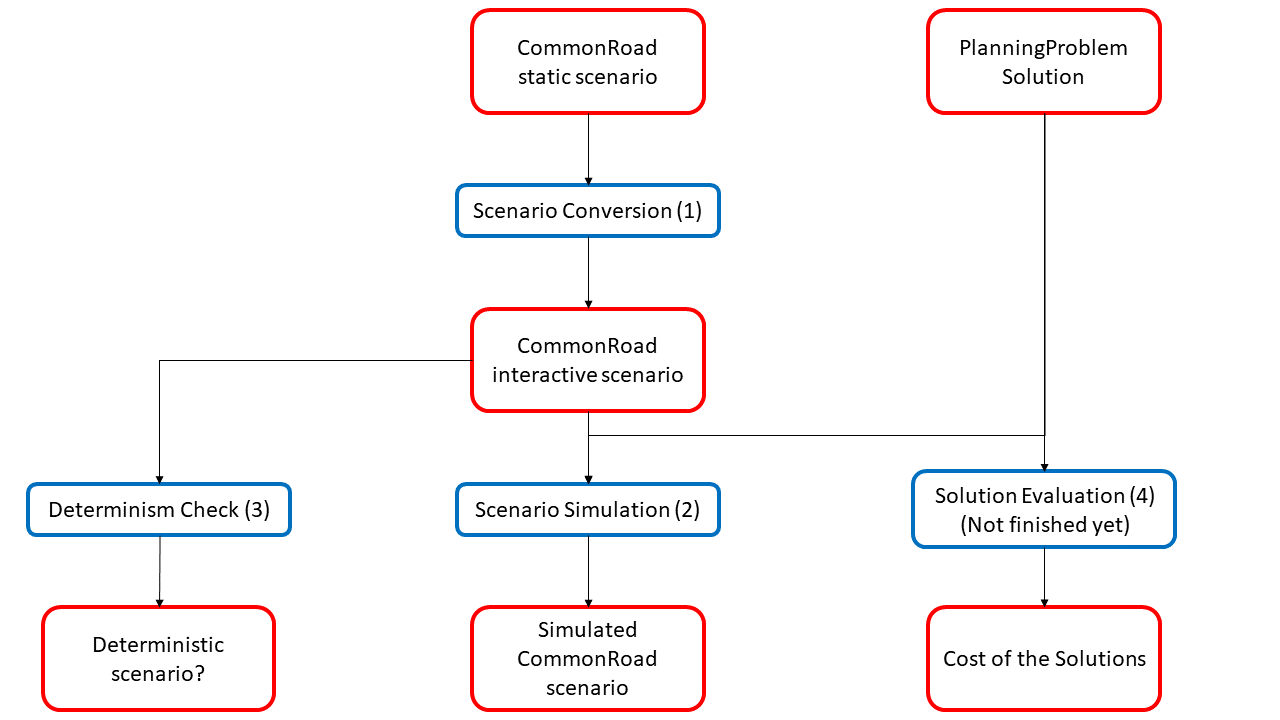
\includegraphics[width = 0.95\linewidth]{fig/fig1.PNG}
    \caption{The functionality and workflow of CommonRoad Interactive Scenarios. Red rectangles are files or variables in Python code, blue rectangles are methods.}
    \label{fig:my_label}
\end{figure}

Then, as demonstrated in Fig. 1, the interactive scenario has the following four functions: Scenario Conversion (1), Scenario Simulation (2), Scenario Determinism Check (3), and Scenario Evaluation (4). Starting from a CommonRoad static scenario, the Scenario Conversion function transforms a static scenario into an interactive scenario. Then the function Scenario Simulation (2) simulates an interactive scenario with/without a given solution, or with a pre-defined motion planner. The results are saved as a simulated CommonRoad scenario locally. The function Determinism Check (3) checks if an interactive scenario is deterministic or not. And the last function Scenario Evaluation quantifies the cost of a solution in an interactive scenario, in order that we can compare different solutions and choose the best one.

\section{Scenario Conversion (1)}
The first function converts a static scenario into an interactive scenario. Figure 2 demonstrates the how the conversion is implemented. First, the scenario is reduced into a scenario with only the initial states and is saved as MapName.cr.xml file. Then the static scenario is converted by the CR2SUMOconverter from the repository \href{https://gitlab.lrz.de/cps/commonroad-map-tool}{CommonRoad map tool}, into a set of SUMO map files. Finally the configurations are saved under the name of `simulation\_config.p’. The combination of all the output files are called an `interactive scenario’.
\begin{figure}[htbp]
    \centering
    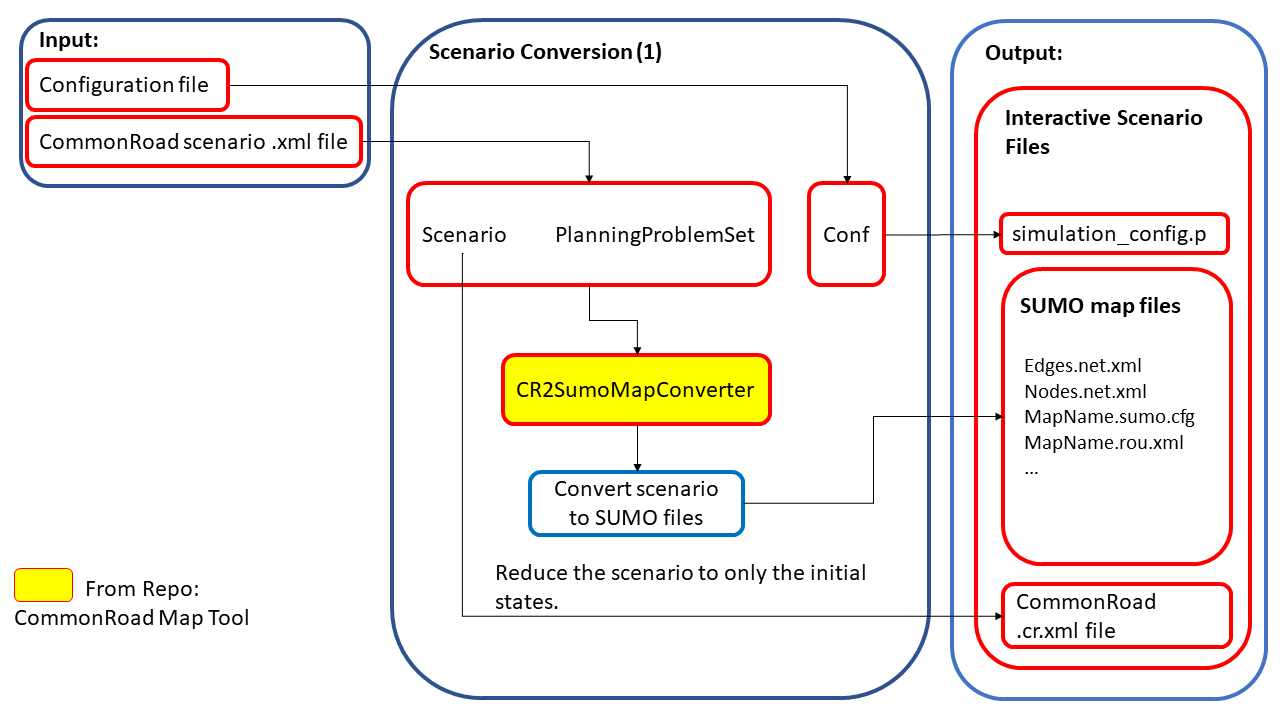
\includegraphics[width = 0.95\linewidth]{fig/fig2.PNG}
    \caption{The workflow of the functionality Scenario Conversion (1)}
    \label{fig:my_label}
\end{figure}

\newpage

The conversion from the vehicle trajectory of the CommonRoad scenario to the vehicle route of the SUMO map vehicles is demonstrated in Fig. 3, we extract the necessary attributes from the initial state and the trajectory of the each vehicle in the CommonRoad scenario, and set the corresponding values in the vehicles' `route' of the SUMO .rou.xml file. For more details it is recommended to understand the implementation of the conversion in the \href{https://gitlab.lrz.de/cps/commonroad-map-tool/-/blob/develop/crmapconverter/sumo_map/cr2sumo/converter.py#L1599}{code}.

\begin{figure}[htbp]
    \centering
    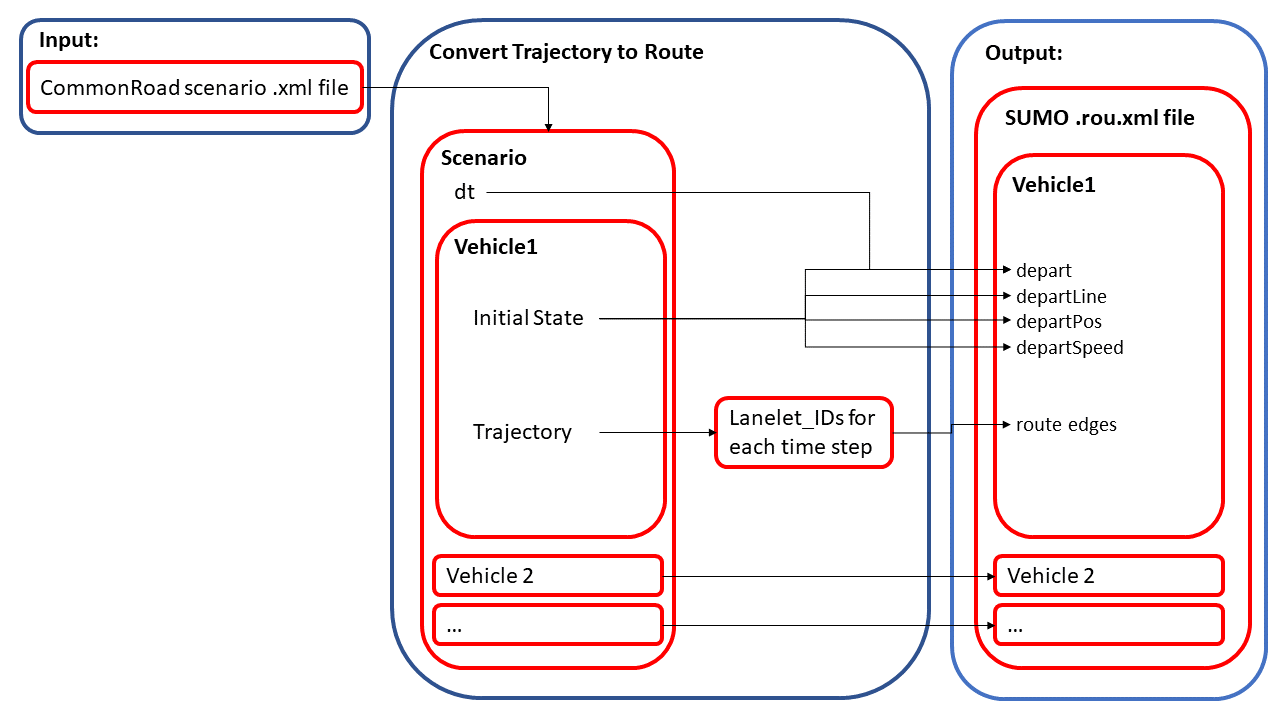
\includegraphics[width = 0.95\linewidth]{fig/fig3.PNG}
    \caption{The workflow of the conversion from CommonRoad scenario trajectory to SUMO route.}
    \label{fig:my_label}
\end{figure}

\newpage

\section{Scenario Simulation (2)}
See Fig. 4. In the function Scenario Simulation (2), firstly we use an AbstractWrapper from the repository \href{https://gitlab.lrz.de/cps/sumo-interface}{SUMO-interface} to collect all the information from the inputs. Then a SumoSimulation is initialized either by connecting the locally installed SUMO with SUMO interface, or by connecting the SUMO simulation in the docker image with the SUMORPCClient from the \href{https://gitlab.lrz.de/cps/commonroad-sumo-manager}{SUMO manager}. *(Now the SUMO Manager repository is already integrated into SUMO-Interface repository) After the initialization of the SumoSimulation, for each time step in the scenario simulation, the code gets the current state of the ego vehicle from the SumoSimulation, updates the state in the next time step if a solution or a motion planner is added, and let the SumoSimulation run the simulation for the next time step. If the simulation succeeds, the simulated CommonRoad scenario can be acquired from the SumoSimulation and saved locally. Optionally, the user can use the Create-gif function from the \href{https://gitlab.lrz.de/cps/sumo-interface}{SUMO-interface} to create a .gif file for the simulated scenario.
\begin{figure}[htbp]
    \centering
    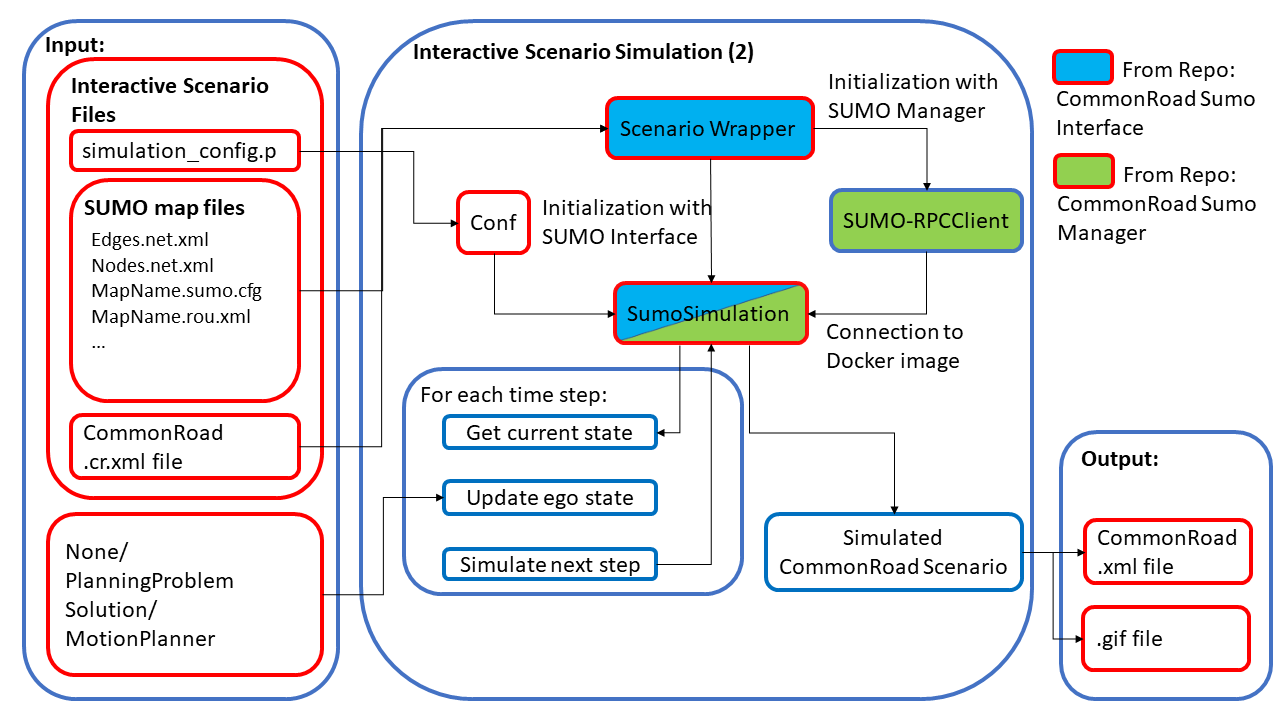
\includegraphics[width = 0.95\linewidth]{fig/fig4.PNG}
    \caption{The workflow of the functionality Scenario Simulation (2)}
    \label{fig:my_label}
\end{figure}

\newpage
\section{Scenario Determinism Check (3)}
See Fig. 5. We check if an interactive scenario is deterministic by checking two things: we resimulate the scenario for several times and check if the simulated scenarios are consistent, and we check the if there are any uncertainties or probabilistic attributes in the MapName.rou.xml file. If and only if the two tests are passed, we say that the interactive scenario is deterministic.
\begin{figure}[htbp]
    \centering
    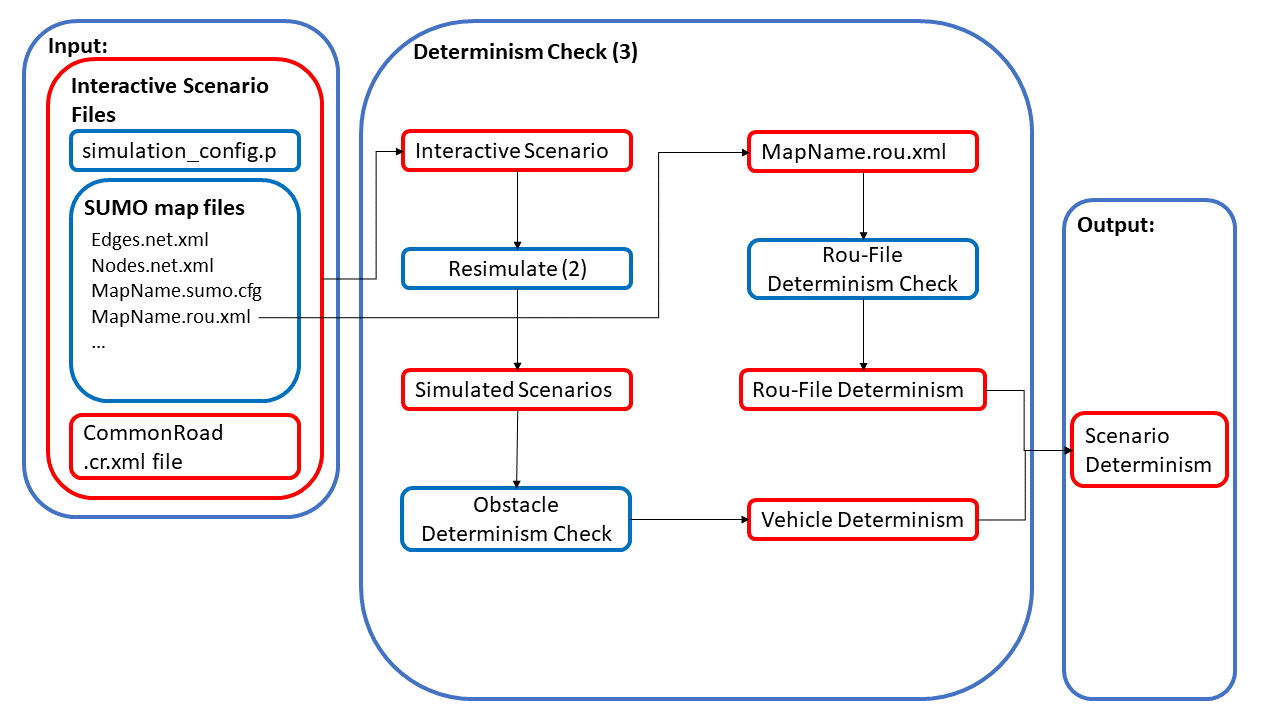
\includegraphics[width = 0.95\linewidth]{fig/fig5.PNG}
    \caption{The workflow of the functionality Scenario Determinism Check (3)}
    \label{fig:my_label}
\end{figure}
\section{Scenario Evaluation (4)}

The idea of the functionality Scenario Evaluation (4) is that, we want to quantify the cost of the solutions so as to compare them horizontally, and see which one is better. The documentation of previous cost functions are \href{https://gitlab.lrz.de/tum-cps/commonroad-cost-functions/-/blob/master/costFunctions_commonRoad.pdf}{here} and a basic framework is already done in \href{https://gitlab.lrz.de/cps/commonroad-interactive-scenarios/-/blob/master/not_for_public_repo/evaluation/evaluate_solution.py}{here}.

\section{SUMO Manager}
SUMO manager is a useful tool with which we can utilize the CommonRoad Interactive Scenario without the local installation of SUMO and SUMO-Interface. 

\subsection{Usage}
\begin{itemize}
    \item Pull the prebuilt docker image from the repository. (If the repository is protected, make sure you have the access and login first before you pull the image. e.g. run \textbf{docker login gitlab.lrz.de:5005/cps/commonroad-sumo-manager} before you pull the docker image by \textbf{docker pull gitlab.lrz.de:5005/cps/commonroad-sumo-manager:ver0.7.2})
    \item Call the function of CommonRoad Interactive Scenarios, and add \textbf{use\_sumo\_manager = True} when calling the function. (If the first time it doesn't work, start a docker container manually first)
    \item Make sure that the \href{https://gitlab.lrz.de/cps/commonroad-sumo-manager/-/blob/master/commonroad_sumo_manager/crsumo/rpc/sumo_client.py#L30}{version} of the client is consistent to the version of the docker image.
\end{itemize}
\subsection{Dockerization}
The docker image of the SUMO Manager is build with the \href{https://gitlab.lrz.de/cps/sumo-interface/sumo_manager_server/Dockerfile}{Dockerfile}. Please follow the instructions there. 
\begin{itemize}
    \item Generate a new \textbf{server.crt} with the command given. When asked for the \textbf{common name}, just enter \textbf{localhost}. (Just English \textbf{localhost}, no numbers.)
    \item Remember to update the generated \textbf{server.crt} \href{https://gitlab.lrz.de/cps/commonroad-sumo-manager/-/tree/master/commonroad_sumo_manager/crsumo/rpc}{here}.
\end{itemize}

\end{document}
